% --------------------------------------------------------------------------------

\section{Introduction} 

\begin{frame}
	
\frametitle{Autoassociative Memories}

\begin{itemize}
    \item Learn to associate a state with itself.
    \item Relax probe towards a learned state.
\end{itemize}

\only<1>{
\begin{center}
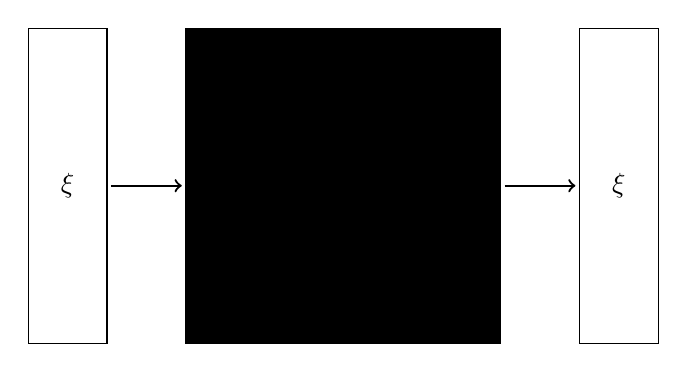
\begin{tikzpicture}
    \draw (0,0) rectangle (1,4);
    \node at (0.5,2) {$\xi$};
    \draw[thick, ->] (1.05,2) --(1.95,2);

    \filldraw[fill=\fillColor, draw=black] (2,0) rectangle (6,4);
    \node[align=center] at (4,2) {Autoassociative\\Memory};
    
    \draw (7,0) rectangle (8,4);
    \node at (7.5,2) {$\xi$};
    \draw[thick, ->] (6.05,2) --(6.95,2);
\end{tikzpicture}
\end{center}
}

\only<2>{
\begin{center}
    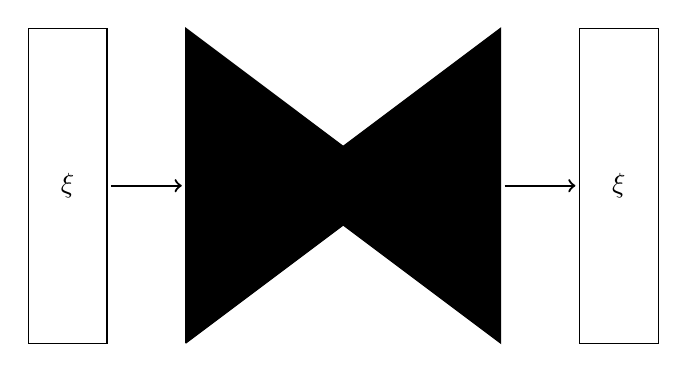
\begin{tikzpicture}
        \draw (0,0) rectangle (1,4);
        \node at (0.5,2) {$\xi$};
        \draw[thick, ->] (1.05,2) --(1.95,2);
    
        \filldraw[fill=\fillColor, draw=black] (2,0) -- (4,1.5) -- (4,2.5) --(2,4) -- (2,0);
        \filldraw[fill=\fillColor, draw=black] (4,1.5) -- (4,2.5) -- (6,4) -- (6,0) -- (4, 1.5);
        
        \draw (7,0) rectangle (8,4);
        \node at (7.5,2) {$\xi$};
        \draw[thick, ->] (6.05,2) --(6.95,2);
    \end{tikzpicture}
\end{center}
}

\only<3>{
\begin{center}
    \begin{tikzpicture}
        \draw (0,0) rectangle (1,4);
        \node at (0.5,2) {$\xi$};

        \draw[thick, ->] (1.05,2) --(6.95,2);
        
        \draw (7,0) rectangle (8,4);
        \node at (7.5,2) {$\xi$};
    \end{tikzpicture}
\end{center}
}

\only<4>{
\begin{center}
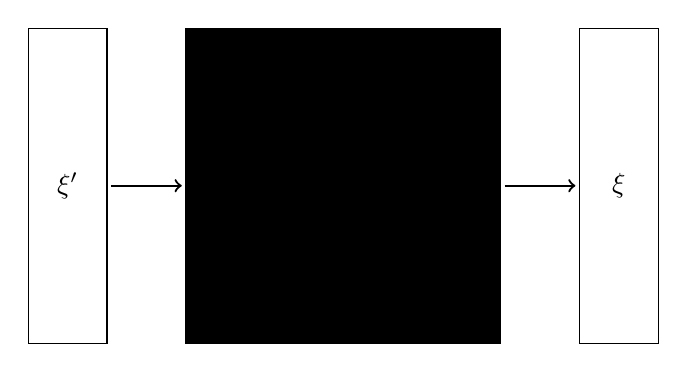
\begin{tikzpicture}
    \draw (0,0) rectangle (1,4);
    \node at (0.5,2) {$\xi^\prime$};
    \draw[thick, ->] (1.05,2) --(1.95,2);

    \filldraw[fill=\fillColor, draw=black] (2,0) rectangle (6,4);
    \node[align=center] at (4,2) {Autoassociative\\Memory};
    
    \draw (7,0) rectangle (8,4);
    \node at (7.5,2) {$\xi$};
    \draw[thick, ->] (6.05,2) --(6.95,2);
\end{tikzpicture}
\end{center}
}
    
\end{frame}

% --------------------------------------------------------------------------------

\subsection{Classical Hopfield Network} 

\begin{frame}
	
    \frametitle{Classical Hopfield Network}
    \begin{columns}[c]
        \column{.6\textwidth}
        \begin{itemize}
            \item Association by Hebbian learning.
            \begin{itemize}
                \item Biological inspiration.
                \item Easy to analyze.
            \end{itemize}
            \item Relax by matrix multiplication.
            \begin{itemize}
                \item Mean field approximation.
                \item Nonlinearity keeps states in bipolar domain.
                \item Energy guaranteed to achieve a minima (under sensible conditions).
            \end{itemize}
        \end{itemize}

        \column{.4\textwidth}
        % TODO Classical Hopfield Image
        \begin{align}
            W &= \sum_{k} \xi_k \otimes \xi_k \\
            \xi_{t+1} &= \text{ Sign}\left( W \cdot \xi_{t} \right) \\
            E \left( \xi \right) &= -\frac{1}{2} \xi^T W \xi
        \end{align}
    \end{columns}
\end{frame}

% --------------------------------------------------------------------------------

\subsection{Modern Hopfield Network} 

\begin{frame}
	
    \frametitle{Modern Hopfield Network}
    \begin{columns}[c]
        \column{.6\textwidth}
        \begin{itemize}
            \item Classical energy wells are too shallow.
            \item Key trick: Replace quadratic energy with general polynomial.
            \begin{itemize}
                \item Heck, anything with a vaguely polynomial shape.
            \end{itemize}
        \end{itemize}

        \begin{align*}
            f_n\left( x \right) &= x^n \\
            f_n\left( x \right) &= \begin{cases}
                x^n \; \text{if } x\geq0 \\
                0 \; \text{if } x<0
            \end{cases} \\
            f_n\left( x \right) &= \begin{cases}
                x^n \; \text{if } x\geq0 \\
                -\epsilon x \; \text{if } x<0
            \end{cases}
        \end{align*}

        \column{.4\textwidth}
        \only<1>{
            \begin{figure}[h]
                \includegraphics[width=\textwidth]{images/introduction_energywell01.png}
            \end{figure}
        }
        \only<2>{
            \begin{figure}[h]
                \includegraphics[width=\textwidth]{images/introduction_energywell02.png}
            \end{figure}
        }
        \only<3>{
            \begin{figure}[h]
                \includegraphics[width=\textwidth]{images/introduction_energywell03.png}
            \end{figure}
        }
        
    \end{columns}
\end{frame}

% --------------------------------------------------------------------------------

\begin{frame}
	
    \frametitle{Modern Hopfield Network}
    \begin{itemize}
        \item New hyperparameter \(n\) -- the ``interaction vertex''.
        \begin{itemize}
            \item Controls the range of influence that memories have.
            \item However, also radically alters the network architecture.
        \end{itemize}

        % TODO: Have visualizations for each of these points comparing either mathematics or visualizations with classical
        \pause
        \item Memory matrix replaced by list of memory states -- vectors of same dimension as data.
        \pause
        \item Learning no longer supports Hebbian -- now requires gradient descent.
        \pause
        \item Relaxation no longer uses mean field -- now a contrastive difference.
        \begin{itemize}
            \item Negative energy no longer means ``stable'' -- the energy \textit{difference} between a neuron clamped on and off indicates stability.
        \end{itemize}
        
    \end{itemize}
\end{frame}